\chapter{Creating a Sketch}

The most basic operation in any sketch-based modeling system is, of course, obtaining a sketch from the user.
The key characteristic of a sketch-capable input device is that it allows freehand input.
While a mouse is capable of this form of input, devices that more closely mimic the feel of freehand drawing using a pen, such as a digitizing tablet, are better for users to maximize their ability to draw.
Devices that serve as both an input device and a display device are particularly suited to this, because it most closely mimics traditional artist creation methods by allowing direct interaction with the sketch space, as opposed to tablets where the space between the input device and the display surface is relative.
Because of this direct interaction method, it is important that our system accurately translated the user's sketch to the 3-D virtual space.
In this chapter we will discuss how we take the sketch input and create a smooth stroke that is independent of the resolution of the input device.

\section{Representation of a Sketch}

At the bare minimum, an input device should provide positional information in some two dimensional coordinate system, usually one based on the interaction window.
For sketch input, the representation must at least approximate continuous movement (Figure~\ref{fig:sampledata}).
Sampling rates vary from one device to the next.
The samples themselves may also be spaced irregularly, with sample points closer as users draw slowly or carefully, or further apart if the user draws quickly.

\begin{figure}
\label{fig:sampledata}
\fbox{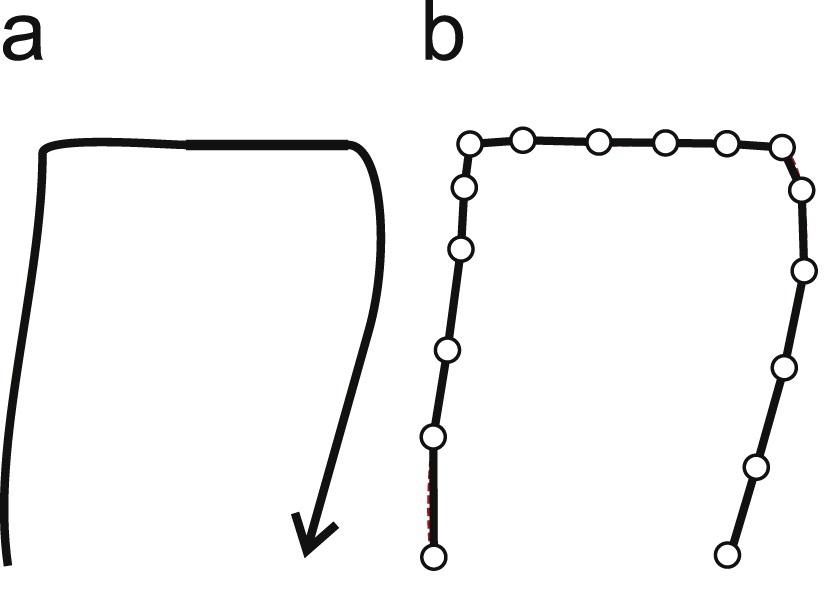
\includegraphics[width=0.98\textwidth]{stroke}}
\caption{An input stroke (a) is provided to the application as (b) a sequence of point samples.}
\end{figure}

We will refer to this sampled sequence of points as a stroke. 
Strokes are stored as a list of points, objects containing coordinates from the sample space, sorted by time.
A sketch is comprised of a large number of these stroke objects.
We also support a simple layer system that can be used to segment a sketch by allowing strokes to be contained in the active layer.


\subsection{Understanding the Stroke Space}
\label{sec:samplespace}

\begin{figure}
\label{fig:samplestroke}
\centering  
\subfigure[The intended complicated stroke input onto a sensing grid.] {\label{fig:sketchintent}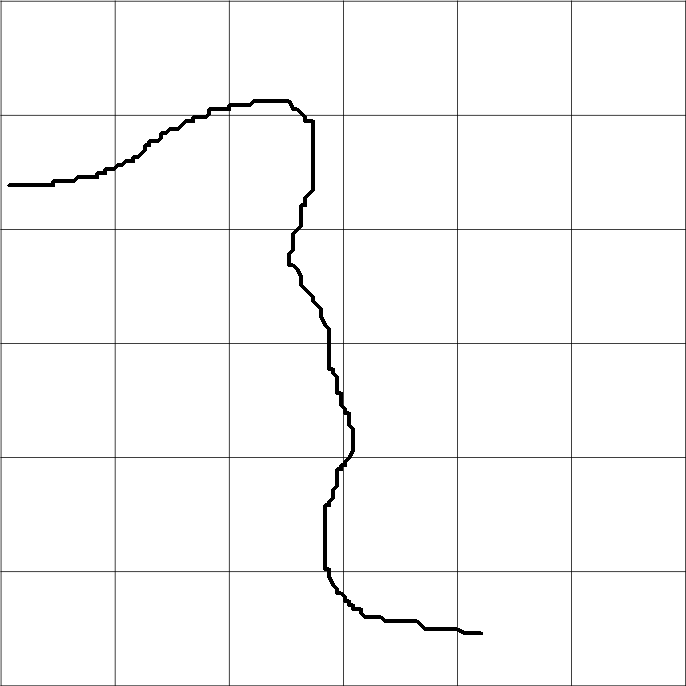
\includegraphics[width=.48\textwidth]{sketchinput}}
\subfigure[A potential raw input detected by the sensor.] {\label{fig:rawinput}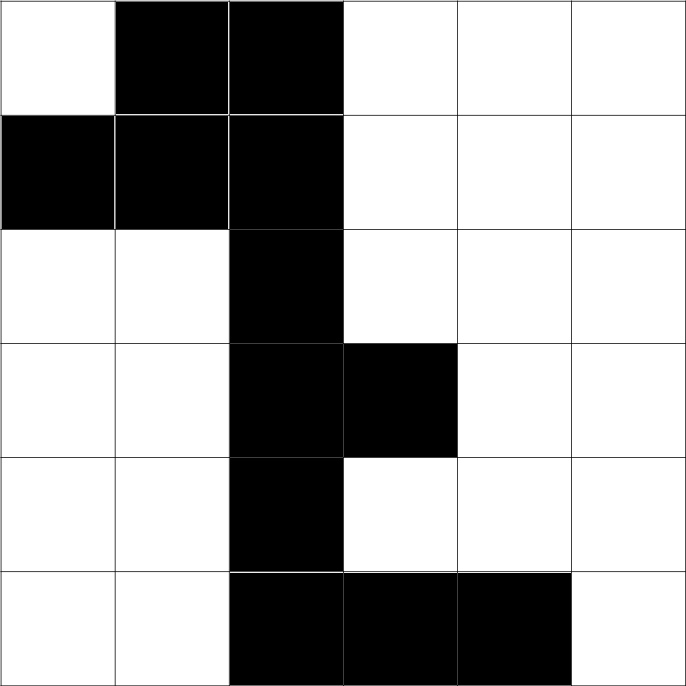
\includegraphics[width=.48\textwidth]{rawinput}}
\caption[Sketch intent versus sketch input]{When sketching, the user's input is rasterized according to the resolution of the sensor. This makes complicated sketch input (a), difficult to understand from the limited resolution of the input (b).}
\end{figure}

Before we discuss how to create smooth strokes, we need to understand how the stroke input gets sent to the application.
When the pen touches the screen, it's position is detected by the touch panel.
This detected position is not necessarily exactly the same as the real world positions of the pen.
This is because the input is rasterized according to the resolution of the sampling device.
For example, assume we are working with integer sample data, and we receive that the pen is at pixel position (148, 148).
The pen could actually be at (147.6, 148.2), or (148.2, 147.6), or any other position that samples to (148, 148) (Figure~\ref{fig:samplestroke}).
This is an issue because in our sketching application, we would like to be able to zoom in to any surface.
This means that small errors in sampling data, and as a result, errors in spline generation, will be magnified.
While the former isn't really an issue, the latter is.


\section{Spline Curves}
\label{sec:splines}

The input data represents an approximation of the stroke input from the user since it is dependent on the sample resolution of the input device, and by extension, the resolution of the display.
Although this would work decently well assuming we are working with a static raster image, three dimensional sketching allows the user to move the camera.
Moving the camera eventually results in poor quality sketches using the stored stroke data due to the lack of sub-sample information that accurately reflects the intent of the original stroke.
To remedy this, a mathematical representation of the curve is needed such that the "sampling rate" of the stroke is independent from the resolution of the input device.
In computer graphics, this is commonly accomplished with spline curves.

A spline is a collection of polynomial segments.
These segments can be linear, cubic, or a polynomial function of any degree.
Splines are a common solution for modeling smooth curves from a small number of points.
For this project, we use a B\'{e}zier curve function for the spline pieces.
A B\'{e}zier curve is a parametric curve commonly used in computer graphics to model infinitely scaling, smooth curves.
The curve is defined by control points $P_0$, $P_1$, ..., $P_n$, and is explicitly evaluated as follows:
\begin{align}
  \mathbf{B}(t) = {} &\sum_{i=0}^n {n\choose i}(1 - t)^{n - i}t^i\mathbf{P}_i \\
                = {} &(1 - t)^n\mathbf{P}_0 + {n\choose 1}(1 - t)^{n - 1}t\mathbf{P}_1 + \cdots \\
                  {} &\cdots + {n\choose n - 1}(1 - t)t^{n - 1}\mathbf{P}_{n - 1} + t^n\mathbf{P}_n,\quad 0 \le t \le 1
\end{align}
where $\scriptstyle {n \choose i}$ are the binomial coefficients, defined as
\begin{equation}
\binom nk = \binom{n-1}{k-1} + \binom{n-1}k \quad \text{for all integers }n,k : 1\le k\le n-1
\end{equation}
with initial values 
\begin{equation}
\binom n0 = \binom nn = 1 \quad \text{for all integers } n\ge0
\end{equation}
The curve can also be evaluated recursively, by
\begin{align}
\mathbf{B}_{\mathbf{P}_0}(t) = \mathbf{P}_0 \\
\mathbf{B}(t) = \mathbf{B}_{\mathbf{P}_0\mathbf{P}_1\ldots\mathbf{P}_n}(t) = (1-t)\mathbf{B}_{\mathbf{P}_0\mathbf{P}_1\ldots\mathbf{P}_{n-1}}(t) + t\mathbf{B}_{\mathbf{P}_1\mathbf{P}_2\ldots\mathbf{P}_n}(t)
\end{align}
What this equation means is that a B\'{e}zier spline of order $n$ can be defined by linear interpolation between two splines of order $n - 1$.
For this project, we will use a cubic B\'{e}zier function for the spline segments.

We must now determine a method for transforming our point sample data to a spline curve.
A naive approach would be to generate a spline curve that passes through the all of our sample points in the sequential order in which they were generated.
Any series of any four distinct points can easily be converted to a cubic B\'{e}zier curve that goes through all four points in the same order.
While this method guarantees that the generated curve passes through all of the input sample points, it is not guaranteed to generate a curve that represents the intent of the original stroke.

\subsection{Generating Splines From the Sample Data}
In theory, creating splines that are accurate to the original stroke would involve generating a curve that passes through each of the sample points.
However in practice, generating a curve in this fashion is not as necessary as one would think. 
As discussed in Section~\ref{sec:samplespace}, the input data that we get is not necessarily accurate to the actual shape of the sketch.
Therefore, even if we were to create a curve that perfectly passed through all of the input points, it is possible that the output curve would still be unsatisfactory.
One common example of this is a user sketching a line diagonally through a screen.
Perfect sample data produces input in a staircase pattern, which would result in a wavy curve not representative of the intent of the original diagonal line (Figure~\ref{fig:staircase}).
Additionally, because the sample distance between points is not consistent, it is possible to produce a curve with artifacts that appear unnatural upon magnification (Figure~\ref{fig:splineartifact}).
What we should actually try to accomplish with our curve generation is to match the intent of the stroke.


The approach we take is using the input samples as control points to generate a piecewise spline curve. 
This method is better at dealing with extreme changes in sample rates because the produced curve contains less convex and concave changes. 
The curve generated will still not pass through the sampled points, but if the sample rate is high, it will ultimately converge or be very close.
Thus using the input data as control points results in smooth reasonable curves even when the control points are far apart.
Additionally, to avoid any "staircase" sampling issues (Figure~\ref{fig:staircaseb}), we include a euclidean distance constraint between the sample data based on the resolution of the input. 
By manipulating the sample data this way, we are able to create curves that reasonably match the intent of the user.

\begin{figure}
\begin{center}
\subfigure[]{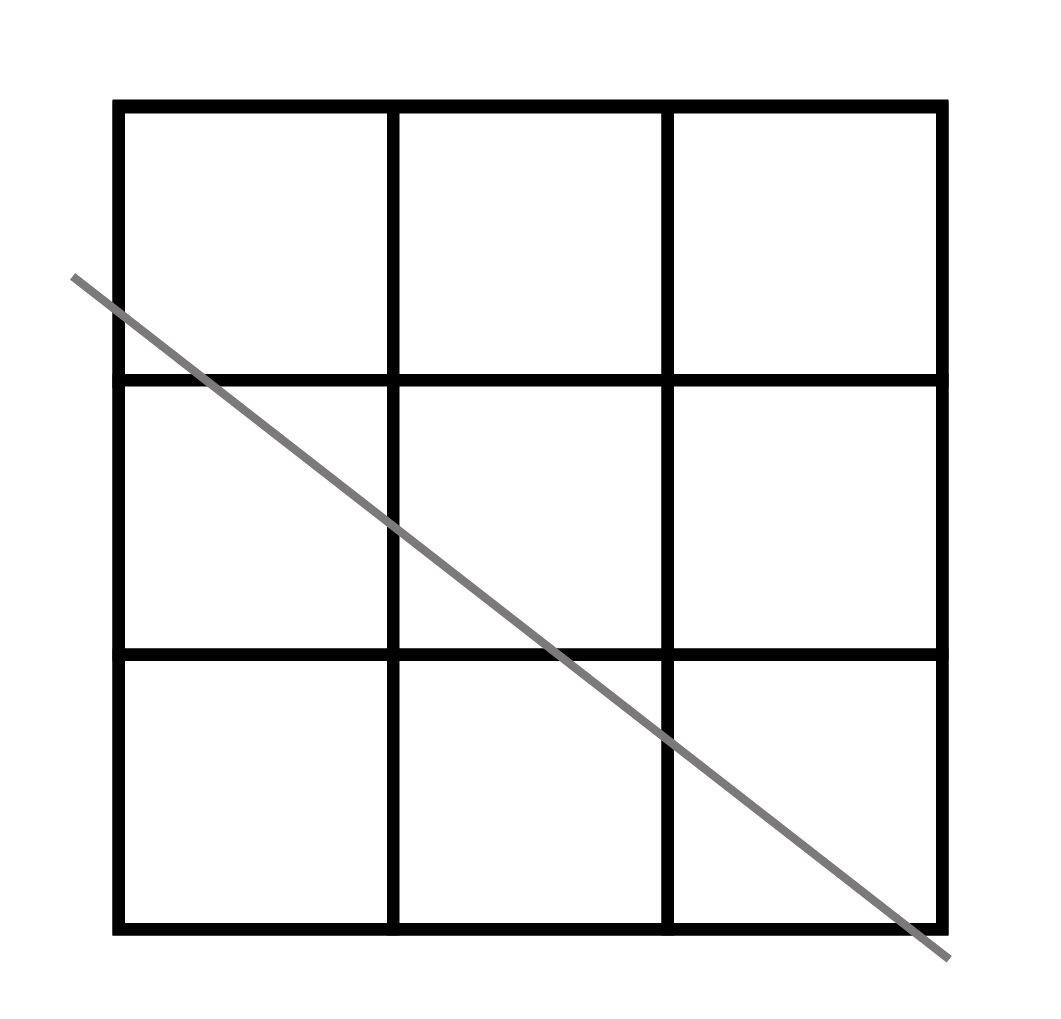
\includegraphics[width=0.32\textwidth]{staircase01.png}}
\subfigure[]{\label{fig:staircaseb}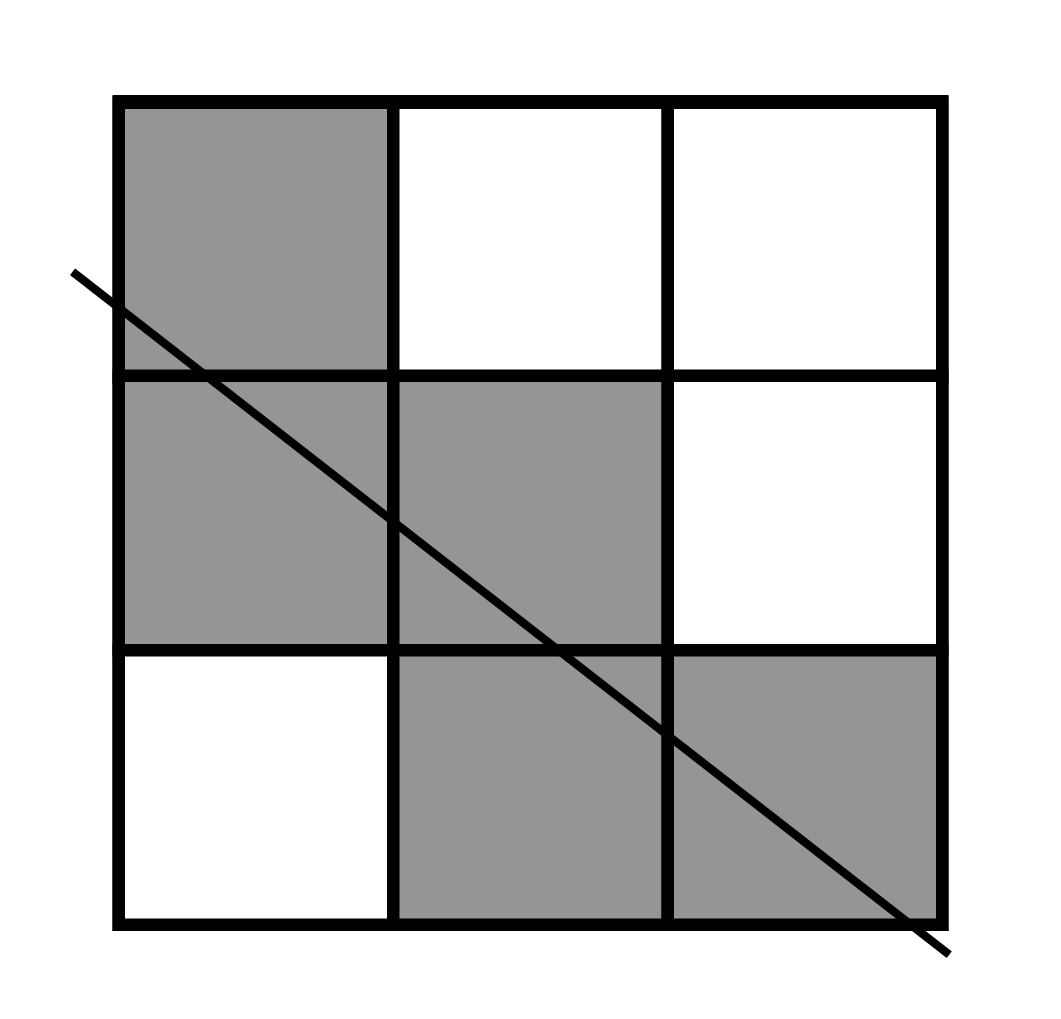
\includegraphics[width=0.32\textwidth]{staircase02.png}}
\subfigure[]{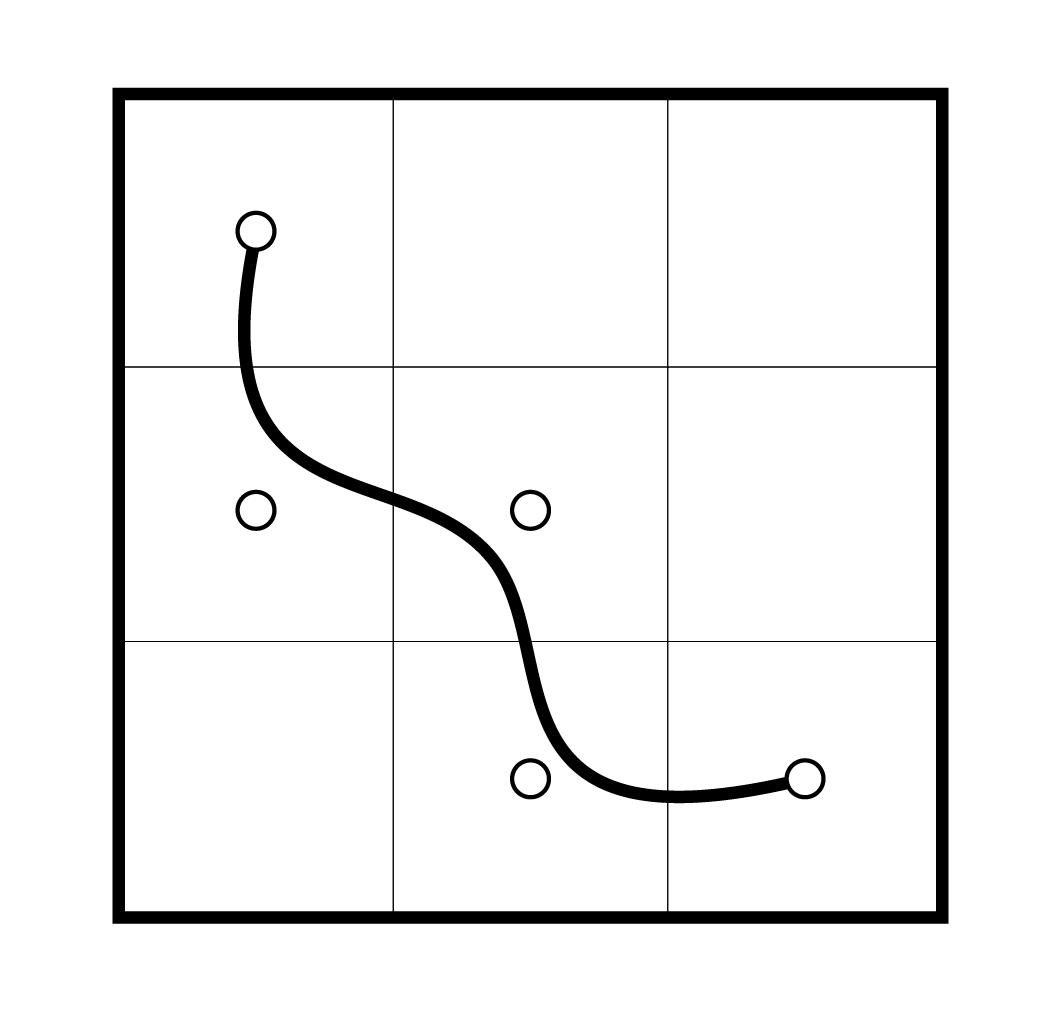
\includegraphics[width=0.32\textwidth]{staircase03.png}}
\end{center}
\caption[Errors in spline generation from how strokes are sampled]{When a diagonal is drawn (a), the input gets rasterized into a staircase pattern of input (b). This input produces curves that do not adequately represent the intent of the original stroke (c). While this effect would be unnoticeable when the diagonal is originally drawn, zooming in onto the curve would reveal the error.}
\label{fig:staircase}
\end{figure}

\begin{figure}
\begin{center}
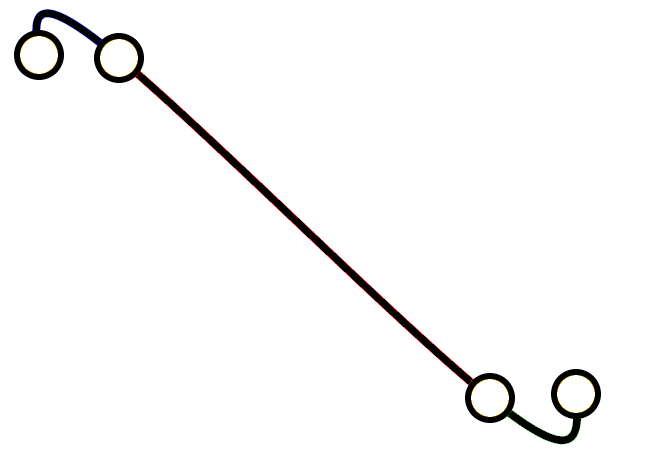
\includegraphics[width=0.6\textwidth]{splineartifact}
\end{center}
\caption[An artifact in spline generation caused by oddly spaced sample points]{Using sample data as geometric knots can result in oddities in the curve generation if the knots have unusual spacing between them. This is very possible because no guarantee is made in the spacing between sampled points.}
\label{fig:splineartifact}
\end{figure}

\subsection{Algorithm}

We begin with a list of control points, numbered from 0 to $N-1$. 
Segment $i$ of the curve is influenced by control points $i-1$, $i$, $i+1$, and $i+2$.
Using this definition we can generate $N-3$ segments from the N control points without falling off the ends of the sequence.

Since we can't render a spline, we need to approximate the curve by subdividing it into small line segments.
We're going to divide each B\'{e}zier curve into a set of connected linear components, with the intent that a large enough number will look sufficiently smooth.
To accomplish this, we use a de Castejau construction, which "splits" a B\'{e}zier curve into two smaller B\'{e}zier curves.
Subdivision of these segments occurs as follows:
\begin{enumerate}
\item Begin with points $\{P_0,P_1,P_2,P_3\}$, which define a B\'{e}zier curve.
\item Define $P_4=(P_0 + P_1)*0.5$, $P_5=(P_1 + P_2)*0.5$, and $P_6=(P_2 + P_3)*0.5$ (Figure~\ref{fig:subdiva})
\item Define $P_7=(P_4 + P_5)*0.5$, and $P_8=(P_5 + P_6)*0.5$ (Figure~\ref{fig:subdivb})
\item Define $P_9=(P_7 + P_8)*0.5$ (Figure~\ref{fig:subdivc})
\item Create two new B\'{e}zier curves using $\{P_0,P_4,P_7,P_9\}$ and $\{P_9,P_8,P_6,P_3\}$ (Figure~\ref{fig:subdivd})
\item Repeat steps 2 through 5 until a termination criteria is met. Possible criteria include distance between control points, and distance between control points $P_1$ and $P_2$ and the line between $P_0$ and $P_3$.
\end{enumerate}
If the termination criteria is small enough, then the curve will appear very smooth, even when zooming in to the curve.
Our termination criteria checks the perpendicular distance between points $P_1$ and $P_2$ and the line the goes through points $P_0$ and $P_3$. (Figure~\ref{fig:subdive})
If both of the distances are below a threshold, the subdivision terminates.
This algorithm produces a smooth B-spline curve starting at control point 0 and ending at $N-1$.

\begin{figure}
\begin{center}
\subfigure[]{\label{fig:subdiva}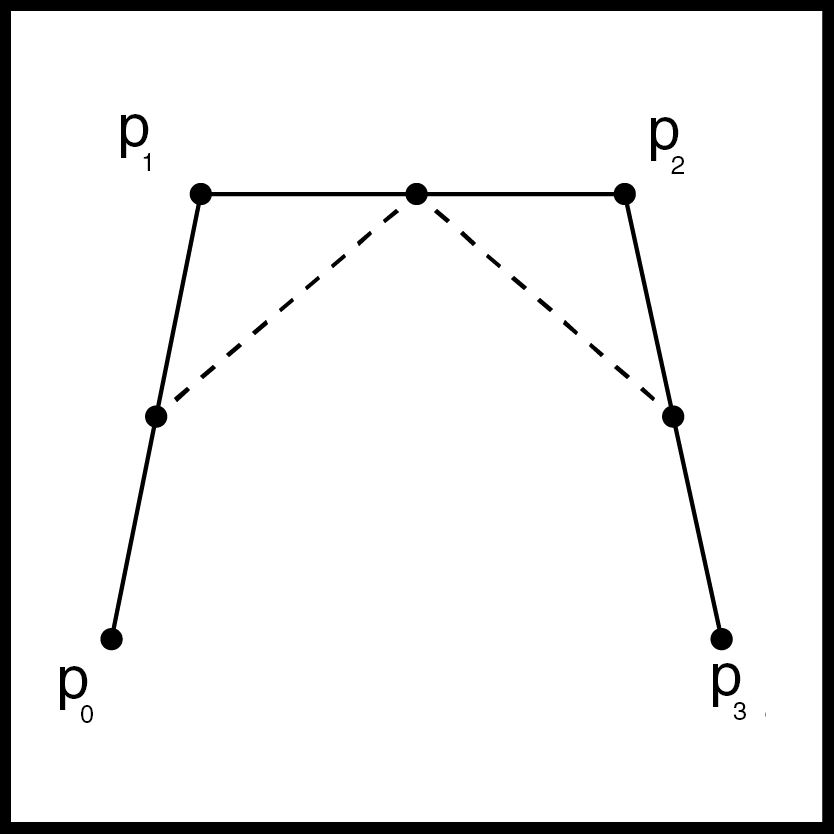
\includegraphics[width=0.32\textwidth]{subdiv1.png}}
\subfigure[]{\label{fig:subdivb}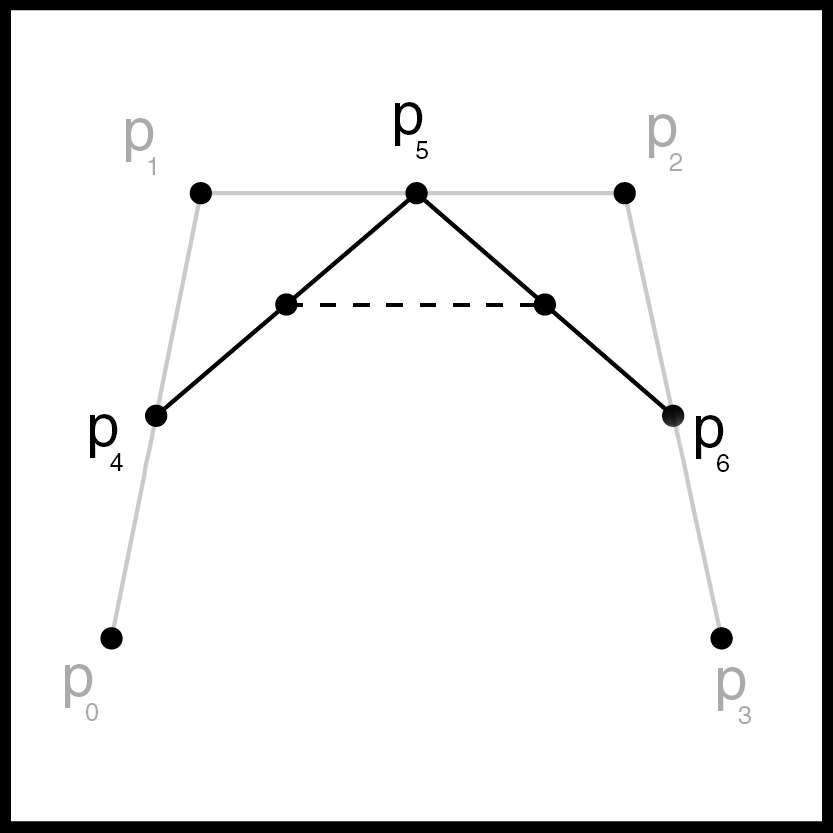
\includegraphics[width=0.32\textwidth]{subdiv2.png}}
\subfigure[]{\label{fig:subdivc}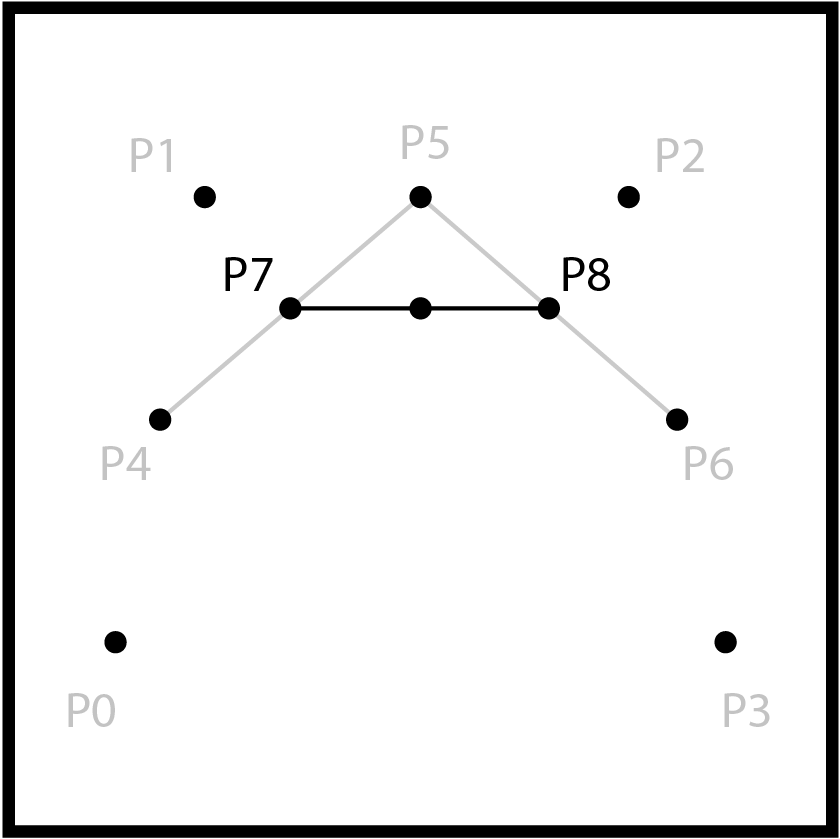
\includegraphics[width=0.32\textwidth]{subdiv3.png}}
\subfigure[]{\label{fig:subdivd}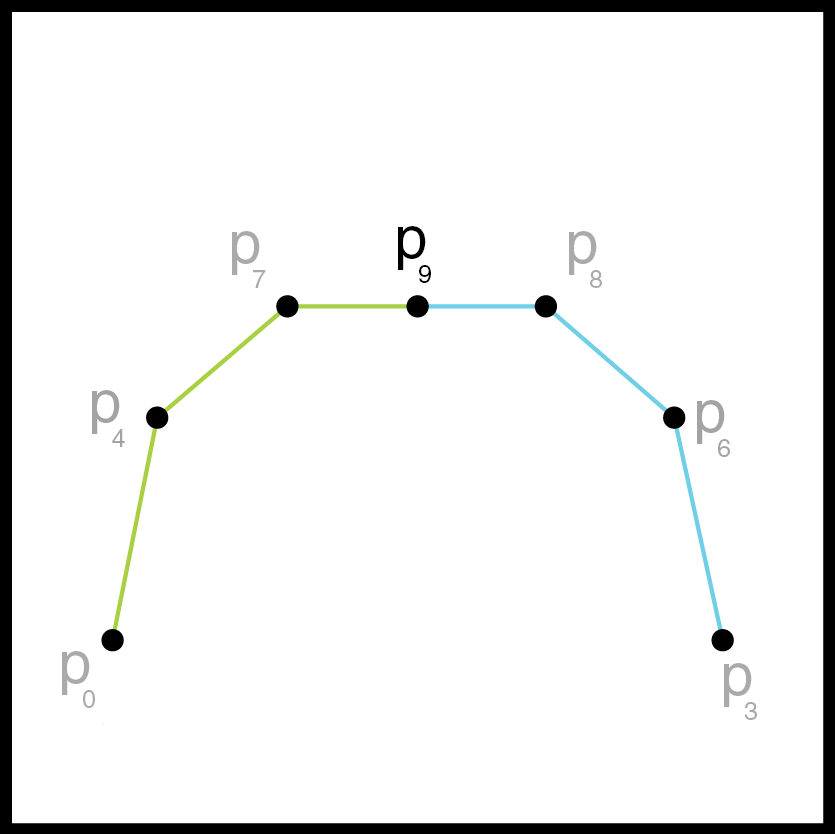
\includegraphics[width=0.32\textwidth]{subdiv5.png}}
\subfigure[]{\label{fig:subdive}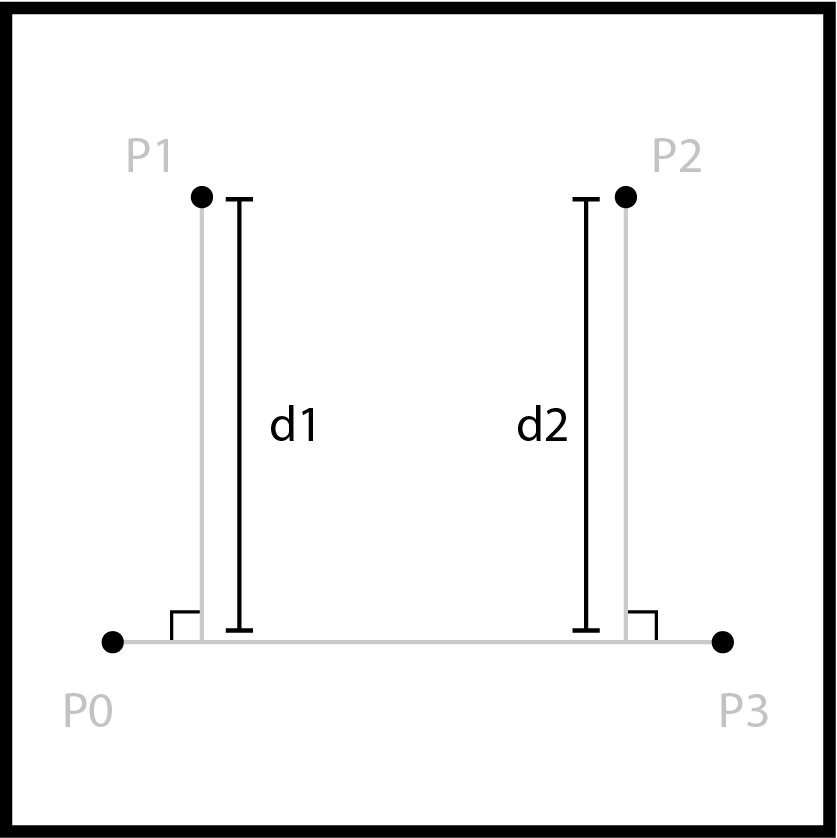
\includegraphics[width=0.32\textwidth]{subdiv4.png}}
\end{center}
\caption[Creating the subdivided polyline from the control points]{We begin with four points representing our spline: $P_0$, $P_1$, $P_2$, and $P_3$. Three points are generated by taking the midpoints of each adjacent segment of the control polygon (a). This process is repeated using the newly created set of points until only one point is generated (b) (c). From the points created through these calculations, two new sets of four points each are created (d). This process is repeated until a termination criteria is reached. We check that the perpendicular distance between two of the control points, $P_1$ and $P_2$, and the line between $P_0$ and $P_3$ is below a certain amount.}
\label{fig:subdiv}
\end{figure}

\section{Summary}
In this section, we described how we convert user input over a set of pixel coordinates into a curve approximating the intent of the stroke.
We believe intent is more important than perfect accuracy since in practice, replicating curves that perfectly match input data results in poor quality curves.
This is because of the finite resolution of a pixel grid, where as in real world sketching, the concept of 'input resolution' does not exist.
Using a B-spline algorithm with cubic B\'{e}zier components, we can calculate a smooth spline curve for our stroke input.